\chapter{Lecture seven: Functions}
\section{Difficulties}

\subsection{Final state for an object}
What happens when an object gets to the final state? Does it die, disappear, or what? \newline \textbf{In analysis:}

\begin{itemize}
    \item The object can no longer perform or suffer events
    \item The state of the object can still be read by a function
\end{itemize}

E.g. a bank account object must exist after we have closed it, so we can read it; e.g. to produce information to the customer and tax authorities at the end of the year. \newline \textbf{In design:}

\begin{itemize}
    \item Decide for how long we'd want to keep objects who are in their final states
    \item E.g. there are laws that define how long a bank account object that is in it's final state (closed) must be kept
\end{itemize}

\subsection{Iteration in state chart diagrams} 

\begin{itemize}
    \item when should we put iteration in the event table and when is it not an iterative event?
    \item How should we describe iteration in the state chart diagram? Should it be through another state and back, or through a loop-arrow?
\end{itemize}

\begin{figure}[H]
    \centering
    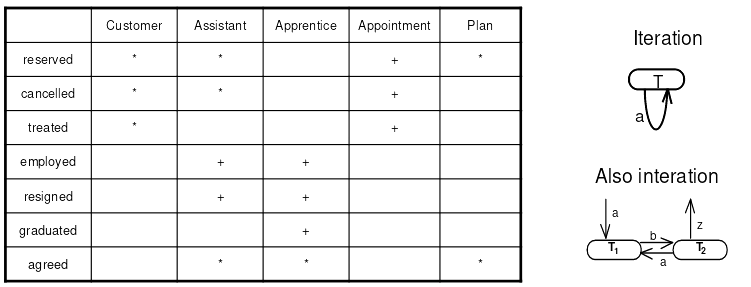
\includegraphics[width=.8\textwidth]{figures/difficultiesiteration.png}
\end{figure}
 

\subsection{Item-Descriptor pattern and the behaviour of the classes} why and when should we use it; and how to we create behavioural patterns for the item and descriptor classes? Generally, it's the distinction between the description/template of the thing, and the instance of the thing.

\begin{figure}[H]
    \centering
    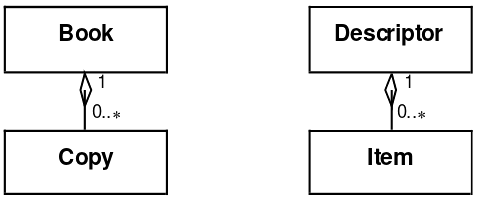
\includegraphics[width=.5\textwidth]{figures/difficultiesitemdescriptor.png}
\end{figure}

\textbf{Events:}
\begin{itemize}
    \item Descriptor: book created, book deleted
    \item Item: copy borrowed, copy returned
    \item Common events: copy bought, copy destroyed
\end{itemize}

\subsection{Actor}
An actor is a user, person, or system interacting with the system that is being developed. Example:

\begin{figure}[H]
    \centering
    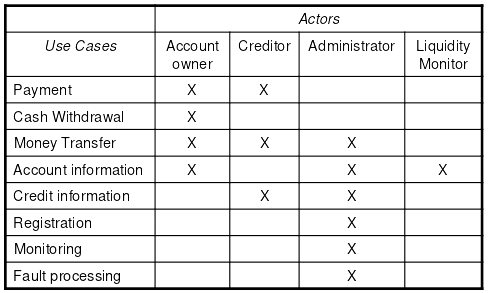
\includegraphics[width=.5\textwidth]{figures/difficultiesactor.png}
\end{figure}

\section{The function activity}
\subsection{Results}
\textbf{Primarily;} a complete list of functions with information of complexity and place of execution. 

\begin{figure}[H]\label{fig:primaryfunctions}
    \centering
    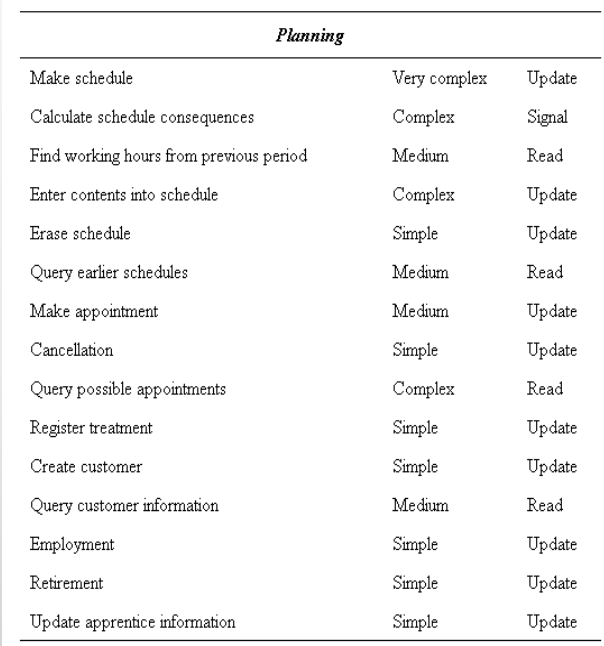
\includegraphics[width=.5\textwidth]{figures/primaryfunctions.png}
\end{figure}

\textbf{Secondarily;} a specification of complex functions with explicit states, and input/output. The aim of this activity is to identify the difficult-to-write functions.

\begin{figure}[H]
    \centering
    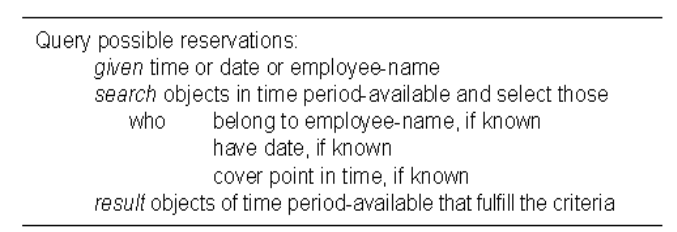
\includegraphics[width=.5\textwidth]{figures/secondaryfunctions.png}
\end{figure}

\subsection{Key concepts}

\subsubsection{Function types}

Function: a facility for making a model useful for actors. A function is activated, executed, and provides a result. Function execution can change a model component's state or create a reaction in the application or problem domains. a function is a requirement. Functions are rarely "pure", but often a combination of more than one of the four types:

\begin{itemize}
    \item \textbf{Update} functions are activated by a problem-domain event and result in a change in the model's state
    \item \textbf{Signal} functions are activated by a change in the model's state and result in a reaction in the context; this might be a display to actors in the AP, or direct intervention in the PD.
    \item \textbf{Read} functions are activated by a need for information in an actor's work task and result in the system displaying relevant parts of the model
    \item \textbf{Compute} functions are activated by a need for information in an actor's work task and consists of a computation with data from the actor or model; result is a display of the computation's result
\end{itemize}

\begin{figure}[H]
    \centering
    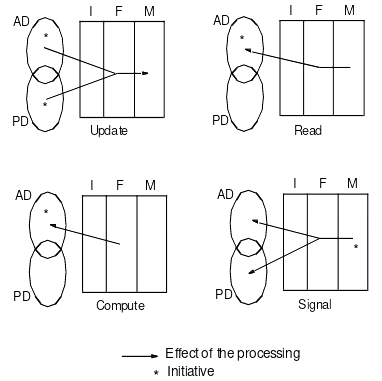
\includegraphics[width=.5\textwidth]{figures/functiontypes.png}
\end{figure}

\subsection{Activities}
The central point of system-functionality analysis is ending with a list of function that is complete and consistent with the use cases. The functions must be consistent with the other analysis results. in particular, functions must support the use cases, and all parts of the model should be used by some function. Only detailed descriptions should be given for the most complex and incomprehensible functions. Three activities in function analysis: Find functions, specify complex functions: and evaluate critically.
\\\textbf{Principles:}
\begin{itemize}
    \item Identify all functions
    \item Specify only complex functions
    \item Check consistency with use cases and the model
\end{itemize}

\begin{figure}[H]
    \centering
    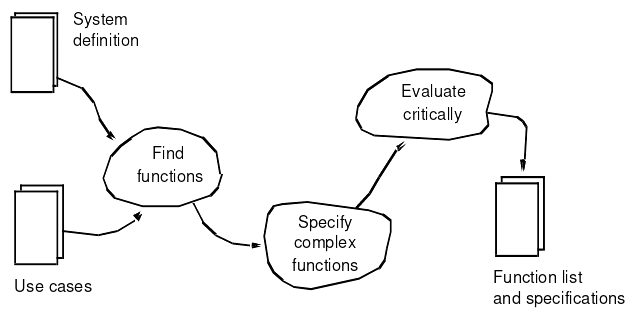
\includegraphics[width=.7\textwidth]{figures/functionsactivities.png}
\end{figure}

\subsubsection{Find functions: Update}
Classes typically give rise to read and update functions. Events lead to requirements for update functions. Use cases give rise to all types of functions. Updating is related to events in the problem domain. For each event ask:

\begin{itemize}
    \item How is the event observed, and how is it registered? In which use cases does this happen?
    \item How should the use cases be supported by update functions?
    \item Which objects, attributes, and object structures are affected by the event, and what requirements does this impose on the update functions?
\end{itemize}

\subsubsection{Find functions: Read}
Classes typically give rise to read and update functions, Use cases give rise to all types of functions. Reading reflects a need for information in the application domain about the problem domain. \\
\textbf{Actor perspective:}
\begin{itemize}
    \item Given the work of the actors, what do the actors need to know about the state of the model? What read functions does this give rise to?
\end{itemize}
\textbf{Model perspective:}
\begin{itemize}
    \item Given the model, which objects and structures will the actors need information about? What read functions does this give rise to?
\end{itemize}

\subsubsection{Find functions: Compute}
Use cases give rise to all types of functions. Computation is used to generate further information. Take your point of departure in actors and use cases:
\begin{itemize}
    \item Which computations (not necessarily based on the model) do the actors need to have carried out?
    \item Does the computational basis come from the actors, the model, or both?
    \item Which computations form complete wholes in the use cases?
\end{itemize}

\subsubsection{Find functions: Signal}
Use cases give rise to all types of functions. Signalling is related to critical states in the model. Examine the model of the problem domain carefully:
\begin{itemize}
    \item What are the critical states for the model?
    \item What is the significance of these critical states? What are the consequences when they occur?
    \item How does a signal function register that the model has entered a critical state?
    \item What signals does each critical state give rise to? How reliable and strong do the signals have to be?
\end{itemize}


\subsubsection{Specify complex functions}
A detailed description might be needed to understand a function sufficiently and to realistically assess its complexity. In most cases this is not necessary during analysis. Basic rule dictates functions should be briefly and informally describes in a list. Only detailed description for special cases. Several methods can be used for this detailed description:

\noindent \textbf{Mathematical expression} can be used, where the relation between input data and output data is specified as $o = f(i)$
\\\textbf{Algorithm} can be described using pseudocode.
\\\textbf{Decomposition} is the further partitioning of a function in the function list, such as the one in figure \ref{fig:primaryfunctions}, showing the complete functional hierarchy directly in the list. A hierarchical function list gives a better overview than a standard list.
\begin{figure}[H]
    \centering
    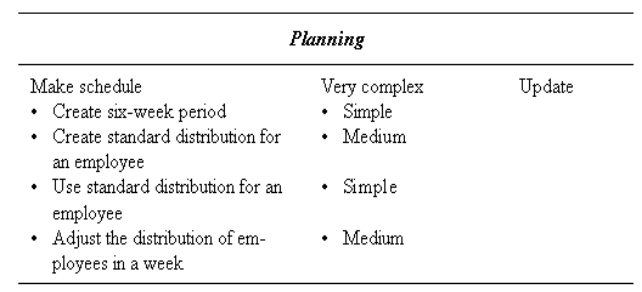
\includegraphics[width=.5\textwidth]{figures/decomposition.png}
\end{figure}

\subsubsection{Evaluate systematically}
There are three ways to ensure that the function list is complete.
Completeness; 
\begin{itemize}
    \item let the users review the list of functions
    \item use the questions for each function type to exhaust that category
    \item compare with the system definition the model, and the use cases
\end{itemize}

Make experiments and prototypes to check the use cases, and to check the set of functions.

\subsection{Functions summary}

\begin{figure}[H]
    \centering
    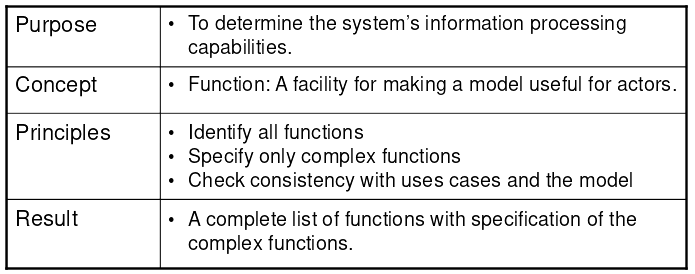
\includegraphics[width=.6\textwidth]{figures/functionssummary.png}
\end{figure}

\section{Challenges in this activity}
\subsection{Appreciate the Difference:Event – Use Case – Function}
See explanation top box page 143 in book.\\ These three are a source of confusion, all three describe dynamic aspects. They are connected but they belong to separate domains. They are all needed because they emphasise different parts of the requirements to the system, but keep them separate.
Example with an order processing system:

\begin{itemize}
    \item Event: Ordered - a customer has entered into a legally binding agreement at a point in time
    \item Use-case: Enter order - a user in the application domain applies the system to make an order for the customer
    \item Function: Create order - in the system's model, an object of the class Order is created
\end{itemize}

\section{Principles}
We can summarise this chapter in three principles for describing functions in object-oriented analysis.

\subsection{Identify all functions}
One of the main purposes of the analysis is to determine the level ambition for the target system. The complete list of functions is an important element in achieving this.

\subsection{Specify only complex functions}
We recommend that you describe the functions briefly and informally in a list. However, it may sometimes be necessary to specify certain functions in detail in order to understand them and assess their complexity.

\subsection{Check consistency with use cases and the model}
The list of functions must be consistent with the list of use cases and the model's classes and events. Checking this can reveal insufficient analysis.